\documentclass[a4paper,UTF8]{article}
\usepackage{ctex}
\usepackage[margin=1.25in]{geometry}
\usepackage{color}
\usepackage{graphicx}
\usepackage{amssymb}
\usepackage{amsmath}
\usepackage{amsthm}
%\usepackage[thmmarks, amsmath, thref]{ntheorem}
\theoremstyle{definition}
\newtheorem*{solution}{Solution}
\newtheorem*{prove}{Proof}
\usepackage{multirow}
\usepackage{url}
\usepackage{enumerate}
\usepackage{algorithm}
\usepackage{algorithmic}
\renewcommand{\algorithmicrequire}{\textbf{Input:}}
\renewcommand{\algorithmicensure}{\textbf{Procedure:}}
\renewcommand\refname{参考文献}

%--

%--
\begin{document}
\title{实验2. 隐马尔科夫模型实践}
\author{MF1733037,刘鑫鑫,\url{xinxliu2014@163.com}}
\maketitle

\section*{综述}
隐马尔科夫模型是一种典型的有向图模型,主要用于时序数据建模。其模型图如下图\ref{fig-1}所示\footnote{图片源于https://cs.nju.edu.cn/wujx/paper/HMM.pdf}。
\begin{figure}[htbp]
\centering
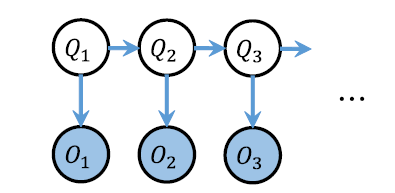
\includegraphics[width=6cm]{1.png}
\caption{隐马尔科夫模型}
\label{fig-1}
\end{figure}
\section*{实验一.}
	\dots

\section*{实验二.}
	\dots

\section*{实验三. }
	\dots

\end{document}